A big part of the data analysis process at the ATLAS trigger system revolves around particle jets. Usually, when working with particle jets, the first action taken is to identify particles that belong to the same jet, namely jet reconstruction. This can provide a link between the observed stable particles and other particles too short-lived to be detected.

%This indirect detection also helps physicists infer properties of those particles, like their mass and spin. Also, through different jet reconstruction methods, physicists measure the total energy before and after a collision in the detector. If it is not what the theory predicts, this could lead to further understanding of physics, beyond the current theories \cite{atkin2015review,hodgkinson2008missing,JetReconstructionAlgorithms}.

Algorithms implementing jet reconstruction are discussed in the first half of this section. These algorithms are the ones chosen for the FastJet software and its performance analysis in chapters \ref{ch:fastjet} and \ref{ch:workfastjet}.  

After the initial jet reconstruction phase, more specialised methods can be applied. One example, jet substructure analysis, is discussed in the second half of this section. Boosted jets, that are comprised of two or more smaller jets (as explained in subsection \ref{ch:fatjet}), are being identified in order to improve the jet reconstruction accuracy. The output of these algorithms is being used as input for the jet reconstruction adversarial neural network discussed in chapters \ref{ch:chann} and \ref{ch:jsann}.


\section{Jet Reconstruction Algorithms}\label{ch:seq_alg}
    A jet reconstruction algorithm is a set of rules that projects a set of particles onto a set of jets \cite{cacciari2012fastjet}. There are various jet reconstruction algorithms developed over the years, aiming to define the kinematics and shape of the jets. There are two main categories: cone algorithms and sequential clustering algorithms.

    Before analysing those two categories, it is worth discussing a property of jet algorithms called Infrared (IR) safety. For algorithms that are IR safe, if two events are almost identical with the exception of the addition of a low energy (soft) particle to one of them, the jets that are reconstructed from each event should also be almost the same. This means that very low energy particles should not essentially contribute to the clustering. A good reconstruction algorithm should therefore be IR safe \cite{algorithms_irc}.% because it is undesirable for fine-details of the detector to have have significant impact on the clustering output .
    
    \subsection{Cone algorithms}
    Cone algorithms assume that particles in jets will show up in conical regions and thus they cluster based on geometry, resulting in jets with rigid circular boundaries (figure \ref{fig:cone}). Differences between various cone algorithms have to do with the strategy taken to search for the stable cones and the procedure used to deal with cases where the same particle is found in multiple stable cones\cite{cacciari2012fastjet}.

\begin{figure}[H]
    \centering
    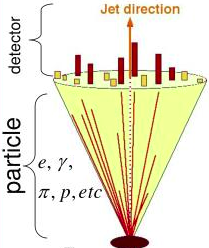
\includegraphics[width=0.4\linewidth]{images/cone_alg.png}
    \caption{Graphical representation of a jet reconstructed using a cone algorithm. All the particles (red lines) included in the conical region are considered part of the jet.}
    \label{fig:cone}
\end{figure}

        In the past, cone algorithms were preferred by physicists as they were more intuitive and easier to implement in a computationally cheap way. However, in the last few years, cone algorithms have tended to be used less and less due to the fact that they are considered to be IR unsafe and that they contain non-physical constants (arbitrary parameters that do not have a meaning in nature). 
        
        Because of their lack of usage, in this project no cone algorithms were selected to work on. This category is presented here for the sake of completeness. 

    \subsection{Sequential Clustering Algorithms}\label{ch:seq}

    Algorithms that belong in the second category, sequential clustering algorithms, assume that particles within jets will have small differences in their momenta and, thus, group particles based on that. 

    Usually the two particles whose momenta are closest together are identified and merged together into one particle. Then the procedure is repeated over and again, until some stopping criterion is reached. The stopping criterion is usually the radius parameter (\textbf{R}), which roughly determines the final size of the jet. The main difference between the various sequential recombination algorithms is their particular choices of distance measure and stopping criterion.  

    Sequential clustering algorithms utilise more physical constants than cone algorithms, and are also IR safe. In the past, algorithms of this type were not favoured as much by physicists because they had slow computational performance. As time progresses, the more optimised versions of algorithms, have resulted in sequential clustering algorithms dominating the particle physics community.
    
    The two most commonly used sequential clustering algorithms are: the anti-$K_t$ and Cambridge/Aachen. The former does a very good job at resolving jets but it is rather difficult to use its results for studying jet substructure. The latter does a good job at resolving jets but its results are much easier to decluster and look for further substructure \cite{atkin2015review}.

\section{Jet substructure algorithms}\label{ch:sub_alg}
As described in chapter \ref{ch:fatjet}, often two or more jets coming from a boosted particle can be so close together that jet reconstruction algorithms find it hard to distinguish between them. One way to deal with this is to treat them as one single fat-jet and apply substructure methods at a later stage. There exists a category of jet variables representing the probability that a particular jet has substructure or what that substructure may be.

\subsection{Substructure variables}\label{ch_sub}

%\verb|https://arxiv.org/pdf/1203.4606.pdf|
\subsubsection{\texorpdfstring{N-subjettiness (${\tau}_{N}$)}{N-subjettiness tau 21)}}
The N-subjettiness variables $\tau_{N}$ are continuous observables related to the subjet multiplicity. Intuitively, the variables can be thought of as answering the question: “How much does this jet look like $N$ different subjets?” \cite{ccetin2012jet}.

The variable $\tau_{N}$ is calculated by re-clustering the constituents of the jet with the kt algorithm and requiring $N$ subjets to be found. Using this definition, this substructure variable describes how well the substructure of the jet is described by $N$ subjets by assessing the degree to which constituents are localised near the axes defined by the kt subjets \cite{ccetin2012jet}.
\subsubsection{\texorpdfstring{$D_2$}{$D_2$}}
$D_2$ investigates how a jet's constituents spread in momentum space and outputs a distribution of probability of this jet consisting of subjets \cite{lectured2}. 